\documentclass[11pt]{article}

\usepackage[latin1]{inputenc}
\usepackage[T1]{fontenc}
\usepackage{graphicx}
\usepackage{float}
\usepackage{amsmath,amssymb,amsfonts}
\usepackage{hyperref}
\usepackage{url}
\usepackage{subfig}
\usepackage{multirow}
\usepackage[a4paper, margin= 2cm]{geometry}
\usepackage{bm}


\usepackage{listings}
\usepackage{pythonhighlight}
\usepackage{color}



\usepackage{amsmath}
\usepackage{textcomp}
\usepackage[top=0.4in, bottom=0.4in, left=0.4in, right=0.4in]{geometry}
% Add other packages here %

\newenvironment{mEnumerate}
{ \begin{enumerate}
    \setlength{\itemsep}{0pt}
    \setlength{\parskip}{0pt}
    \setlength{\parsep}{0pt}     }
{ \end{enumerate}                  } 


% Put your group number and names in the author field %
\title{\bf Exercise 1.\\ Implementing a first Application in RePast: A Rabbits Grass Simulation.}
\author{Group \textnumero 29 \\ Student 1, 298032 \\ Student 2, 293330}

\begin{document}
\maketitle

\section{Implementation}

\subsection{Assumptions}
% Describe the assumptions of your world model and implementation (e.g. is the grass amount bounded in each cell) %

We make multiple assumptions about the world and the behavior of the agents (furthermore referred to as \textit{rabbits} or \textit{agents}), namely:

\begin{mEnumerate}
    \item the world consists of rabbits (the agents) and grass (environment),
    \item the world is a 2d-grid of equal length in both dimensions,
    \item only the rabbits can move, only one cell at the time, and only one cell (Manhatten distance of 1),
    \item moving one cell cost one energy
    \item there is no boundary, the two-dimensional world is topologically equivalent to a Torus,
    \item only one rabbit can exist per cell (thus limiting the total number of rabbits),
    \item a rabbit will not make a move into an occupied cell, if no space is free, rabbit will stay and not consume any energy
    \item the world enforces a strict and constant order of actions (see \ref{sec:implementation-remarks})
    \item rabbits can reproduce and will do so regardless of available space, doing so will transfer some energy to the offspring (set by \texttt{InitRabbitEnergy}, the cost to reproduce is defined by \texttt{BirthThreshold}, this amount of energy will be reduced from the agent upon reproduction),
    \item rabbits will only reproduce once every tick,
    \item rabbits don't have a limited lifespan, however they die if they don't have any energy left at the end of the tick.
    \item the grass growth is not limited, each round a fixed amount of grass grows randomly distributed on the grid
\end{mEnumerate}

\subsection{Implementation Remarks}\label{sec:implementation-remarks}
% Provide important details about your implementation, such as handling of boundary conditions %

The actions that the rabbits perform, or that happen in the world, follow a constant order and are executed sequentially. Meaning that first all rabbits move, then they all eat, etc. This list defined as:

\begin{mEnumerate}
    \item Shuffling of agents
    \item \begin{mEnumerate}
        \item Agents move. Each agent moves one after the other, if one agent can't move he stays fixed.
        \item Agents eat
        \item Agents reproduce
        \item Agents die
        \item Grass grows
    \end{mEnumerate}
\end{mEnumerate}

\section{Results}
In the following experiments you'll see a plot consisting of three subplots. From left to right: Initial parameters, world view at the end of the experiment (the darker the green the more grass, white indicating no grass, a red square indicating an agent on this cell), and a plot listing the total number of alive agents in red, the total energy of the agents in blue and the total amount of grass in turquoise.

The default grid size of 20 was not altered in any experiment.

% In this section, you study and describe how different variables (e.g. birth threshold, grass growth rate etc.) or combinations of variables influence the results. Different experiments with different settings are described below with your observations and analysis

\subsection{Experiment 1}

\begin{figure}[H]
 \begin{center}
  \includegraphics[width=0.8\textwidth]{plots/fewerRabbits&lessGrass.PNG}
  \caption{Small amount of initial agents and grass leading to a dead world.}
  \label{fig:experiment1}
 \end{center}
\end{figure}


\subsubsection{Setting}
In the first experiment, we initialized the model with a low number of rabbits of 5, a low grass growth rate of 1, a low initial energy of 5 and a high birth threshold of 100.

\subsubsection{Observations}
% Elaborate on the observed results %
Given the high birth threshold and low grass growth the rabbits die out quickly, as indicated in the population plot of Figure \ref{fig:experiment1}. Since all rabbits are dead the grass can grow freely and will turn the world green.

\subsection{Experiment 2}

\begin{figure}[H]
 \begin{center}
  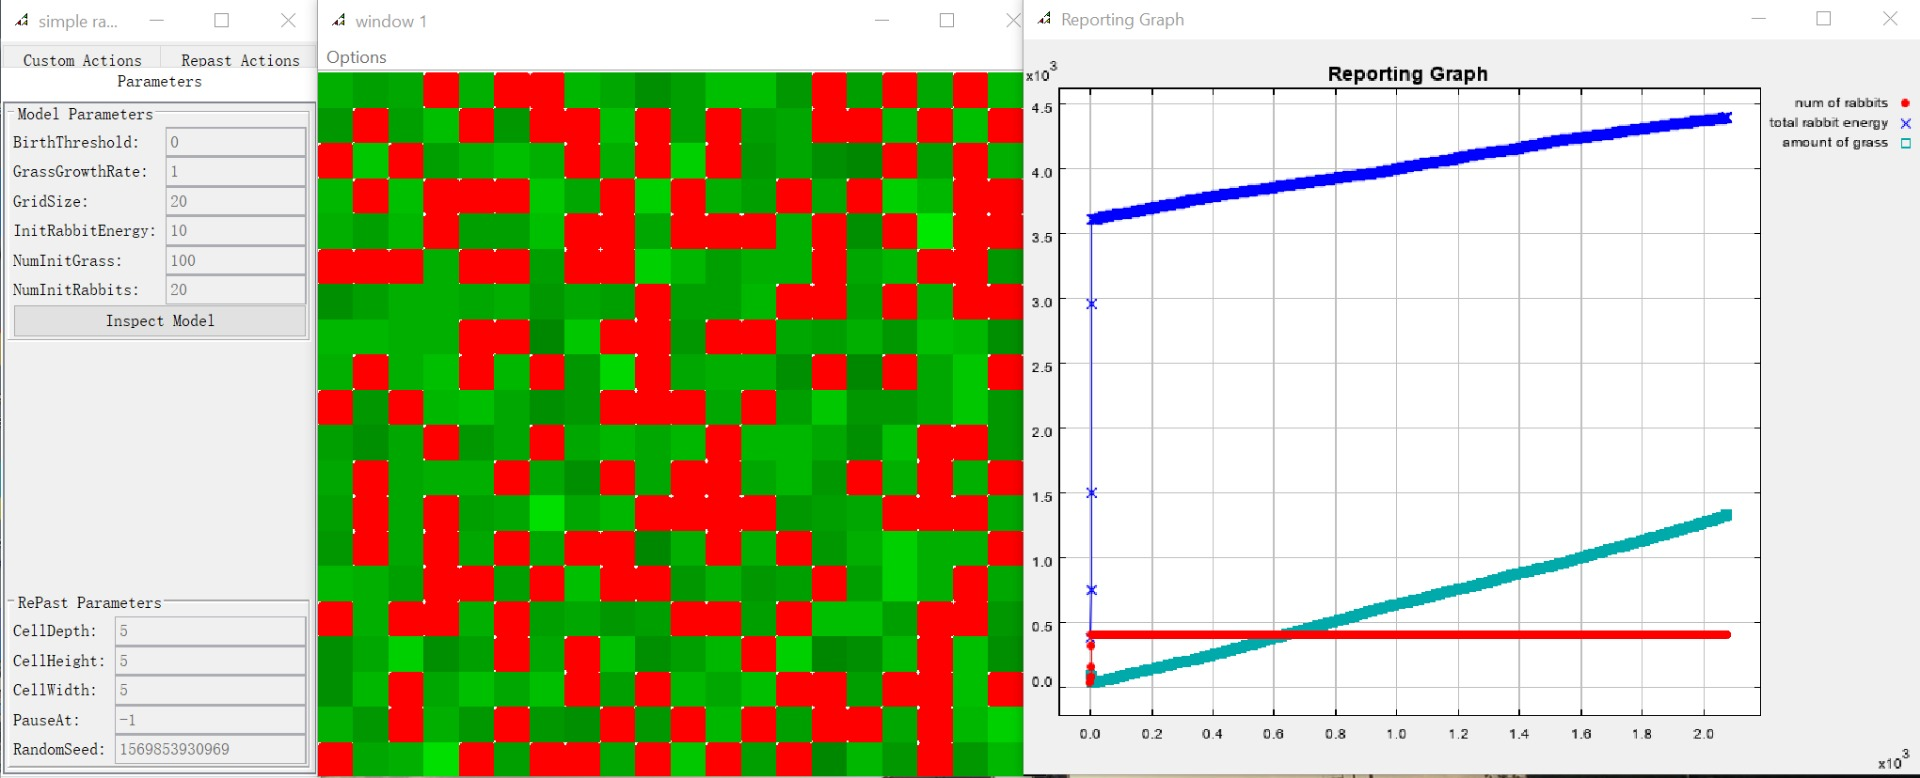
\includegraphics[width=0.8\textwidth]{plots/noBirthThreshould.jpeg}
  \caption{Zero energy cost of reproduction give rise to world filled with rabbits}
  \label{fig:experiment2}
 \end{center}
\end{figure}

\subsubsection{Setting}
In the second experiment, we initialized the model with 20 rabbits, 10 units of initial energy and 100 units of grass, and a birth threshold of 0.


\subsubsection{Observations}
% Elaborate on the observed results %
As there is no energy cost for reproduction in this experiment, the number of rabbits grows exponentially, saturating the world with rabbits in a few ticks, as can be seen in Figure \ref{fig:experiment2}.

\subsection{Experiment 3}

\begin{figure}[H]
 \begin{center}
  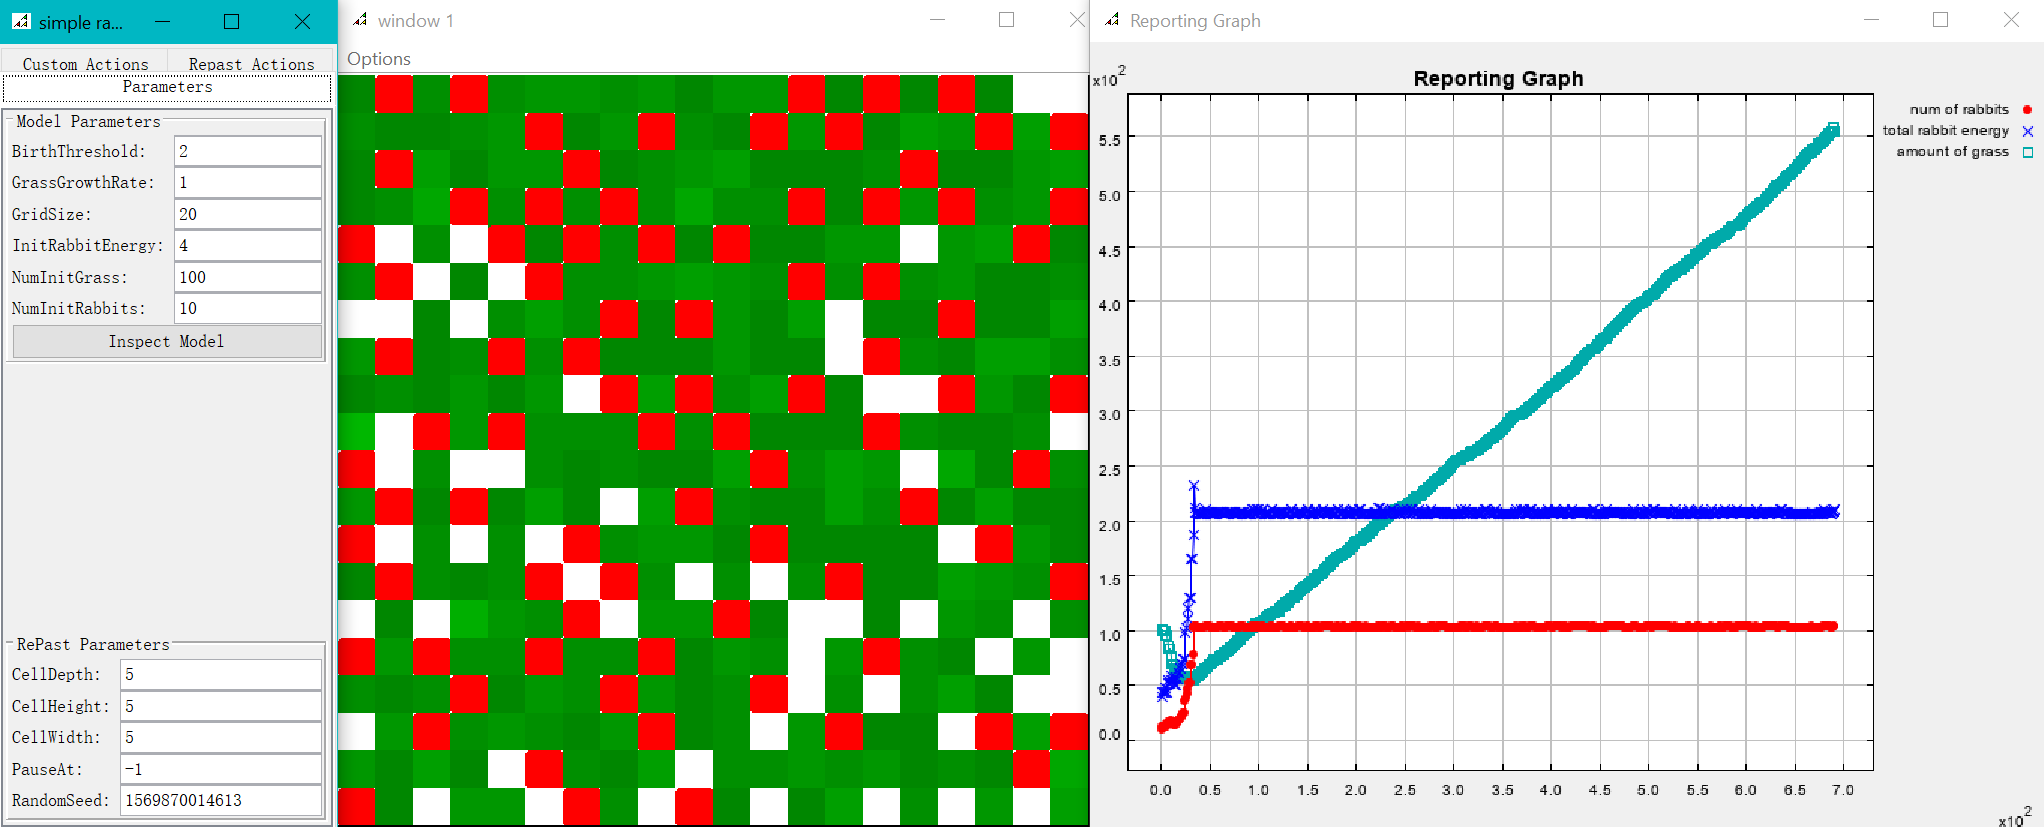
\includegraphics[width=0.8\textwidth]{plots/balance1.PNG}
  \caption{Simulations when population of rabbits converges to a limited value}
  \label{fig:experiment3}
 \end{center}
\end{figure}

\subsubsection{Setting}
In the third experiment, we start with 10 rabbits, each initialized with 4 units of energy. The reproduction will cost 2 units of energy (making the reproduction process to produce energy instead of consuming it). There are 100 units of grass provided and the grass will grow with rate 1.

\subsubsection{Observations}
% Elaborate on the observed results %
Given the high initial supply of grass, the low reproduction cost, and the higher initial energy the rabbit population reaches a fluctuating equilibrium around 100 alive rabbits, as can be seen in Figure \ref{fig:experiment3}.

\end{document}
